\section{Lecture 20: Angular Momentum, Continued}

Is is obvious that:
\[ [hat{x}_i, \hat{p}_j] = i \hbar \delta_{ij}, [hat{x}_i, \hat{x}_j] = [hat{p}_i, \hat{p}_j] = 0 \]
We showed last time that:
\[ [\hat{L}_i, \hat{L}_j] = i \hbar \hat{L}_k \delta_{ij}, [\hat{L}^2, \hat{L}_z] = 0 \]

We typically describe the state with two quantum numbers:
\[ \hat{L}^2, \hat{L}_z \to \ket{\ell m}  \]

Use a right-handed coordinate system to define polar coordinate system.

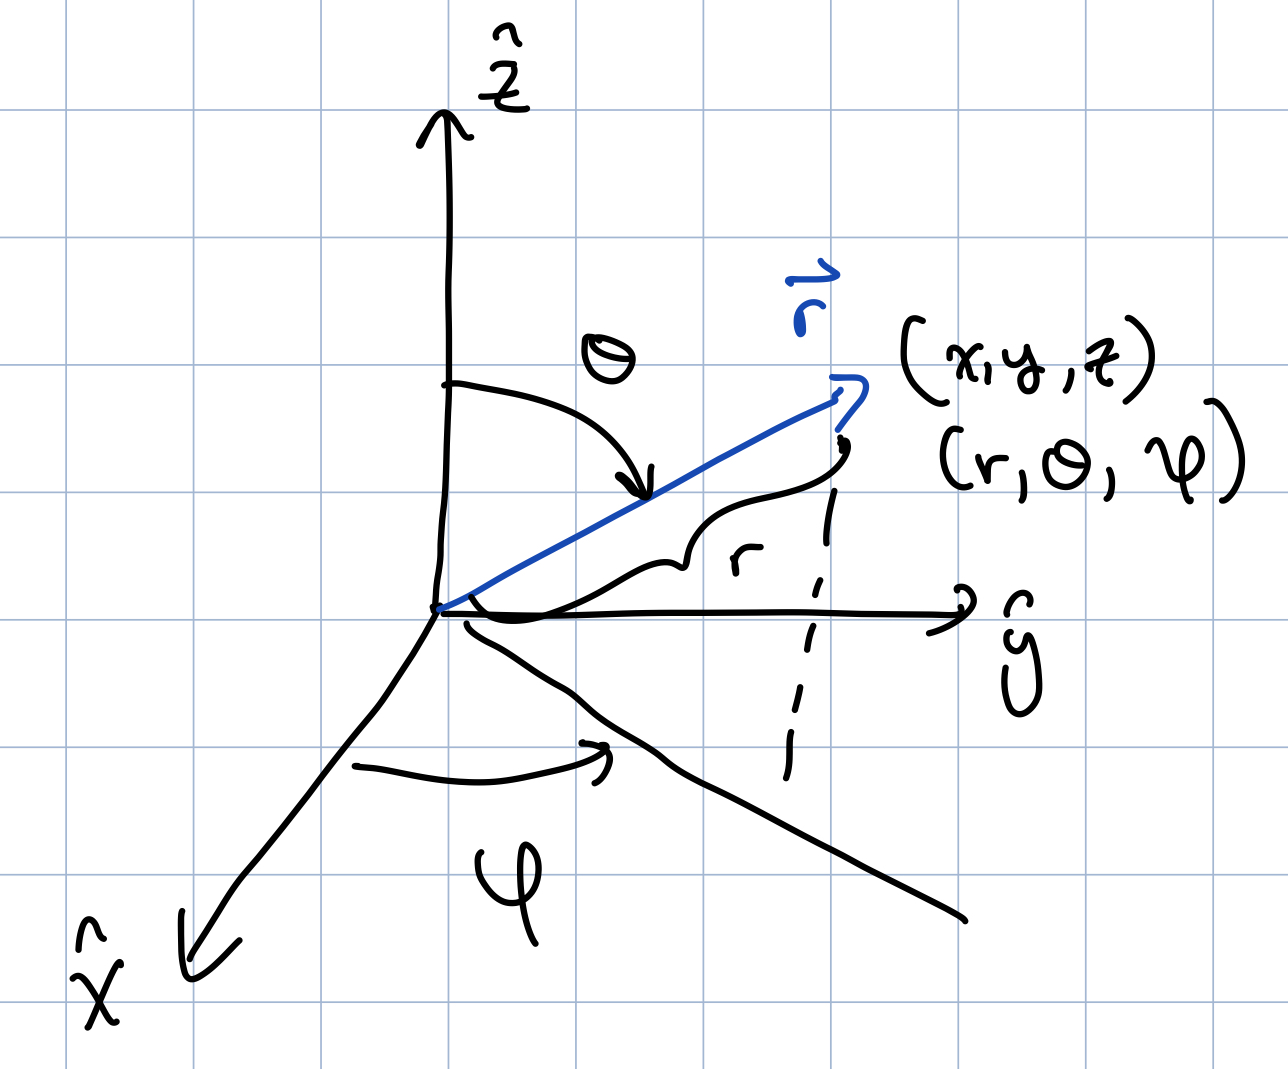
\includegraphics[width=300px]{spherical.jpeg}

The ranges of these coordinates are:
\[ (r, \theta, \varphi) \in [0, \infty] \times [0, \pi] \times [0, 2\pi]\]

The angular momentum operators look like:
\begin{align*}
    \hat{L}_x &= -i\hbar\qty(- \sin \varphi \pdv{}{\theta} - \cot \theta \cos \varphi \pdv{}{\varphi}) \\
    \hat{L}_y &= -i\hbar\qty(- \cos \varphi \pdv{}{\theta} - \cot \theta \sin \varphi \pdv{}{\varphi}) \\
    \hat{L}_z &= -i\hbar \pdv{}{\varphi} \\
    \hat{L}^2 &= -\hbar^2\qty[\frac{1}{\sin \theta} \pdv{}{\theta} \qty(\sin \theta \pdv{}{\theta}) + \frac{1}{\sin^2\theta} \pdv{^2}{\varphi^2}]
\end{align*}

where notice $r$ is missing, i.e.:
\[ \comm{\hat{L}_i}{f(r)} = 0 \]

\begin{theorem}[Generators of Rotations]
    To generate a finite rotation $\alpha$ about a unit vector $\hat{n}$:
    \[ \hat{U}_{\hat{n}}(\alpha) = \exp\qty(- \frac{i}{\hbar} \alpha \hat{n} \cdot \hat{L})\]

    To generate a infinitesimal rotation $\delta \alpha$, we can linearize to:
    \[ \hat{U}_{\hat{n}}(\delta\alpha) = \hat{I} - \frac{i}{\hbar} \delta\alpha \hat{L}_z\]
\end{theorem}

\subsection{Eigenfunctions and Eigenvalues of Angular Momentum}
Niels Bohr told us that angular momentum was quantized for atomic orbitals, i.e. $mvr = n \hbar$ for mass $m$ and integral $n$

Call an eigenfunction of the $\hat{L}_z$ operator: $\Phi_m(\varphi)$ with eigenvalue $m \hbar$.
\[ \hat{L}_z \Phi_m(\varphi) = m \hbar \Phi_m(\varphi) \]
This yields a differential equation:
\begin{align*}
    -i \pdv{}{\varphi} \Phi_m(\varphi) &= m \Phi_m(\varphi) \\
    \Phi_m(\varphi) &= \frac{1}{\sqrt{2\pi}}
\end{align*}

A clear boundary condition is:
\begin{align*}
    \Phi_m(2\pi + \varphi) &= \Phi_m(\varphi) \\
    e^{2\pi i m} &= 1 \\
    m &\in \Z
\end{align*}
So angular momentum must be quantized! Furthermore, $\Phi_m$ form a complete orthonormal basis for functions of $\phi$.
\[ f(\varphi) = \sum_{m \in \Z} a_m \Phi_m(\varphi) \]
Employing Fourier's trick:
\[ a_m = \int_{0}^{2\pi} \Phi_{m}^* (\varphi) f(\varphi) \dd{\varphi} \]

Call a separable eigenfunction of the $\hat{L}^2$ as $Y_{\ell m}(\theta, \varphi) = \Theta_{\ell m}(\theta) \Phi_m(\varphi)$, the spherical harmonic. Note that this is
also an eigenfunction for $\hat{L}_z$.

